% Options for packages loaded elsewhere
\PassOptionsToPackage{unicode}{hyperref}
\PassOptionsToPackage{hyphens}{url}
\PassOptionsToPackage{dvipsnames,svgnames,x11names}{xcolor}
%
\documentclass[
  12pt,
  a4paper,
  DIV=11,
  numbers=noendperiod]{scrartcl}

\usepackage{amsmath,amssymb}
\usepackage{iftex}
\ifPDFTeX
  \usepackage[T1]{fontenc}
  \usepackage[utf8]{inputenc}
  \usepackage{textcomp} % provide euro and other symbols
\else % if luatex or xetex
  \usepackage{unicode-math}
  \defaultfontfeatures{Scale=MatchLowercase}
  \defaultfontfeatures[\rmfamily]{Ligatures=TeX,Scale=1}
\fi
\usepackage{lmodern}
\ifPDFTeX\else  
    % xetex/luatex font selection
\fi
% Use upquote if available, for straight quotes in verbatim environments
\IfFileExists{upquote.sty}{\usepackage{upquote}}{}
\IfFileExists{microtype.sty}{% use microtype if available
  \usepackage[]{microtype}
  \UseMicrotypeSet[protrusion]{basicmath} % disable protrusion for tt fonts
}{}
\makeatletter
\@ifundefined{KOMAClassName}{% if non-KOMA class
  \IfFileExists{parskip.sty}{%
    \usepackage{parskip}
  }{% else
    \setlength{\parindent}{0pt}
    \setlength{\parskip}{6pt plus 2pt minus 1pt}}
}{% if KOMA class
  \KOMAoptions{parskip=half}}
\makeatother
\usepackage{xcolor}
\usepackage[top=30mm,left=25mm,right=25mm,bottom=30mm,heightrounded]{geometry}
\setlength{\emergencystretch}{3em} % prevent overfull lines
\setcounter{secnumdepth}{-\maxdimen} % remove section numbering
% Make \paragraph and \subparagraph free-standing
\makeatletter
\ifx\paragraph\undefined\else
  \let\oldparagraph\paragraph
  \renewcommand{\paragraph}{
    \@ifstar
      \xxxParagraphStar
      \xxxParagraphNoStar
  }
  \newcommand{\xxxParagraphStar}[1]{\oldparagraph*{#1}\mbox{}}
  \newcommand{\xxxParagraphNoStar}[1]{\oldparagraph{#1}\mbox{}}
\fi
\ifx\subparagraph\undefined\else
  \let\oldsubparagraph\subparagraph
  \renewcommand{\subparagraph}{
    \@ifstar
      \xxxSubParagraphStar
      \xxxSubParagraphNoStar
  }
  \newcommand{\xxxSubParagraphStar}[1]{\oldsubparagraph*{#1}\mbox{}}
  \newcommand{\xxxSubParagraphNoStar}[1]{\oldsubparagraph{#1}\mbox{}}
\fi
\makeatother


\providecommand{\tightlist}{%
  \setlength{\itemsep}{0pt}\setlength{\parskip}{0pt}}\usepackage{longtable,booktabs,array}
\usepackage{calc} % for calculating minipage widths
% Correct order of tables after \paragraph or \subparagraph
\usepackage{etoolbox}
\makeatletter
\patchcmd\longtable{\par}{\if@noskipsec\mbox{}\fi\par}{}{}
\makeatother
% Allow footnotes in longtable head/foot
\IfFileExists{footnotehyper.sty}{\usepackage{footnotehyper}}{\usepackage{footnote}}
\makesavenoteenv{longtable}
\usepackage{graphicx}
\makeatletter
\def\maxwidth{\ifdim\Gin@nat@width>\linewidth\linewidth\else\Gin@nat@width\fi}
\def\maxheight{\ifdim\Gin@nat@height>\textheight\textheight\else\Gin@nat@height\fi}
\makeatother
% Scale images if necessary, so that they will not overflow the page
% margins by default, and it is still possible to overwrite the defaults
% using explicit options in \includegraphics[width, height, ...]{}
\setkeys{Gin}{width=\maxwidth,height=\maxheight,keepaspectratio}
% Set default figure placement to htbp
\makeatletter
\def\fps@figure{htbp}
\makeatother
% definitions for citeproc citations
\NewDocumentCommand\citeproctext{}{}
\NewDocumentCommand\citeproc{mm}{%
  \begingroup\def\citeproctext{#2}\cite{#1}\endgroup}
\makeatletter
 % allow citations to break across lines
 \let\@cite@ofmt\@firstofone
 % avoid brackets around text for \cite:
 \def\@biblabel#1{}
 \def\@cite#1#2{{#1\if@tempswa , #2\fi}}
\makeatother
\newlength{\cslhangindent}
\setlength{\cslhangindent}{1.5em}
\newlength{\csllabelwidth}
\setlength{\csllabelwidth}{3em}
\newenvironment{CSLReferences}[2] % #1 hanging-indent, #2 entry-spacing
 {\begin{list}{}{%
  \setlength{\itemindent}{0pt}
  \setlength{\leftmargin}{0pt}
  \setlength{\parsep}{0pt}
  % turn on hanging indent if param 1 is 1
  \ifodd #1
   \setlength{\leftmargin}{\cslhangindent}
   \setlength{\itemindent}{-1\cslhangindent}
  \fi
  % set entry spacing
  \setlength{\itemsep}{#2\baselineskip}}}
 {\end{list}}
\usepackage{calc}
\newcommand{\CSLBlock}[1]{\hfill\break\parbox[t]{\linewidth}{\strut\ignorespaces#1\strut}}
\newcommand{\CSLLeftMargin}[1]{\parbox[t]{\csllabelwidth}{\strut#1\strut}}
\newcommand{\CSLRightInline}[1]{\parbox[t]{\linewidth - \csllabelwidth}{\strut#1\strut}}
\newcommand{\CSLIndent}[1]{\hspace{\cslhangindent}#1}

\KOMAoption{captions}{tableheading}
\usepackage{fancyhdr}
\pagestyle{fancy}
\fancyhead[L]{MSc ENR ISM: Exercise C}
\fancyhead[C]{}
\fancyhead[R]{Marius King, May 03, 2025}
\makeatletter
\@ifpackageloaded{caption}{}{\usepackage{caption}}
\AtBeginDocument{%
\ifdefined\contentsname
  \renewcommand*\contentsname{Table of contents}
\else
  \newcommand\contentsname{Table of contents}
\fi
\ifdefined\listfigurename
  \renewcommand*\listfigurename{List of Figures}
\else
  \newcommand\listfigurename{List of Figures}
\fi
\ifdefined\listtablename
  \renewcommand*\listtablename{List of Tables}
\else
  \newcommand\listtablename{List of Tables}
\fi
\ifdefined\figurename
  \renewcommand*\figurename{Figure}
\else
  \newcommand\figurename{Figure}
\fi
\ifdefined\tablename
  \renewcommand*\tablename{Table}
\else
  \newcommand\tablename{Table}
\fi
}
\@ifpackageloaded{float}{}{\usepackage{float}}
\floatstyle{ruled}
\@ifundefined{c@chapter}{\newfloat{codelisting}{h}{lop}}{\newfloat{codelisting}{h}{lop}[chapter]}
\floatname{codelisting}{Listing}
\newcommand*\listoflistings{\listof{codelisting}{List of Listings}}
\makeatother
\makeatletter
\makeatother
\makeatletter
\@ifpackageloaded{caption}{}{\usepackage{caption}}
\@ifpackageloaded{subcaption}{}{\usepackage{subcaption}}
\makeatother

\ifLuaTeX
  \usepackage{selnolig}  % disable illegal ligatures
\fi
\usepackage{bookmark}

\IfFileExists{xurl.sty}{\usepackage{xurl}}{} % add URL line breaks if available
\urlstyle{same} % disable monospaced font for URLs
\hypersetup{
  colorlinks=true,
  linkcolor={blue},
  filecolor={Maroon},
  citecolor={Blue},
  urlcolor={Blue},
  pdfcreator={LaTeX via pandoc}}


\author{}
\date{}

\begin{document}


\section{Ecological Indicator Values and Functional
Traits}\label{ecological-indicator-values-and-functional-traits}

\subsection{Methods}\label{methods}

The analysis is based on vegetation survey data from Swiss grasslands
(meadows and lawns), consisting of plot-wise species abundance data and
corresponding header information. From the header data, only the landuse
classification was used.

\subsubsection{Community Means of Ecological Indicator
Values}\label{community-means-of-ecological-indicator-values}

Ecological indicator values (EIVs) for Europe were obtained from Dengler
et al. (2023) and matched to the species list of the vegetation data.
Species that could not be matched directly were checked for taxonomic
discrepancies and corrected when possible. Species without available
EIVs or with uncertain identification at the species or genus level were
excluded prior to analysis.

Community means of EIVs were calculated at the plot level without
abundance weighting. Differences in community means between meadows and
lawns were analyzed statistically and visualized with boxplots.

\subsubsection{Community-Weighted Means of Functional
Traits}\label{community-weighted-means-of-functional-traits}

Functional trait data, specifically canopy height, seed mass, and
specific leaf area (SLA), were sourced from the LEDA trait database
(Kleyer et al. 2008). Trait datasets were merged and inspected for
skewness; values for canopy height and seed mass were log₁₀-transformed
to approximate normal distributions. As with the EIVs, trait data were
matched to the species list, and species lacking trait information or
with uncertain identification were excluded.

Community-weighted means (CWMs) of the functional traits were calculated
using the \texttt{functcomp} function from the FD package (Laliberté and
Legendre 2010; Laliberté, Legendre, and Shipley 2014), weighting trait
values by species abundances. Differences between meadows and lawns were
statistically tested and visualized using boxplots.

All analyses were performed in R version 4.5.0 (R Core Team 2025).

\subsection{Results}\label{results}

A significant difference in the community ecological indicator values
(EIVs) was found for nitrogen between meadows and lawns, with meadows
exhibiting higher mean nitrogen values
(Figure~\ref{fig-eiv_unweighted}). Temperature values tended to be
higher in meadows as well, but the difference was not statistically
significant.

\begin{figure}[H]

\centering{

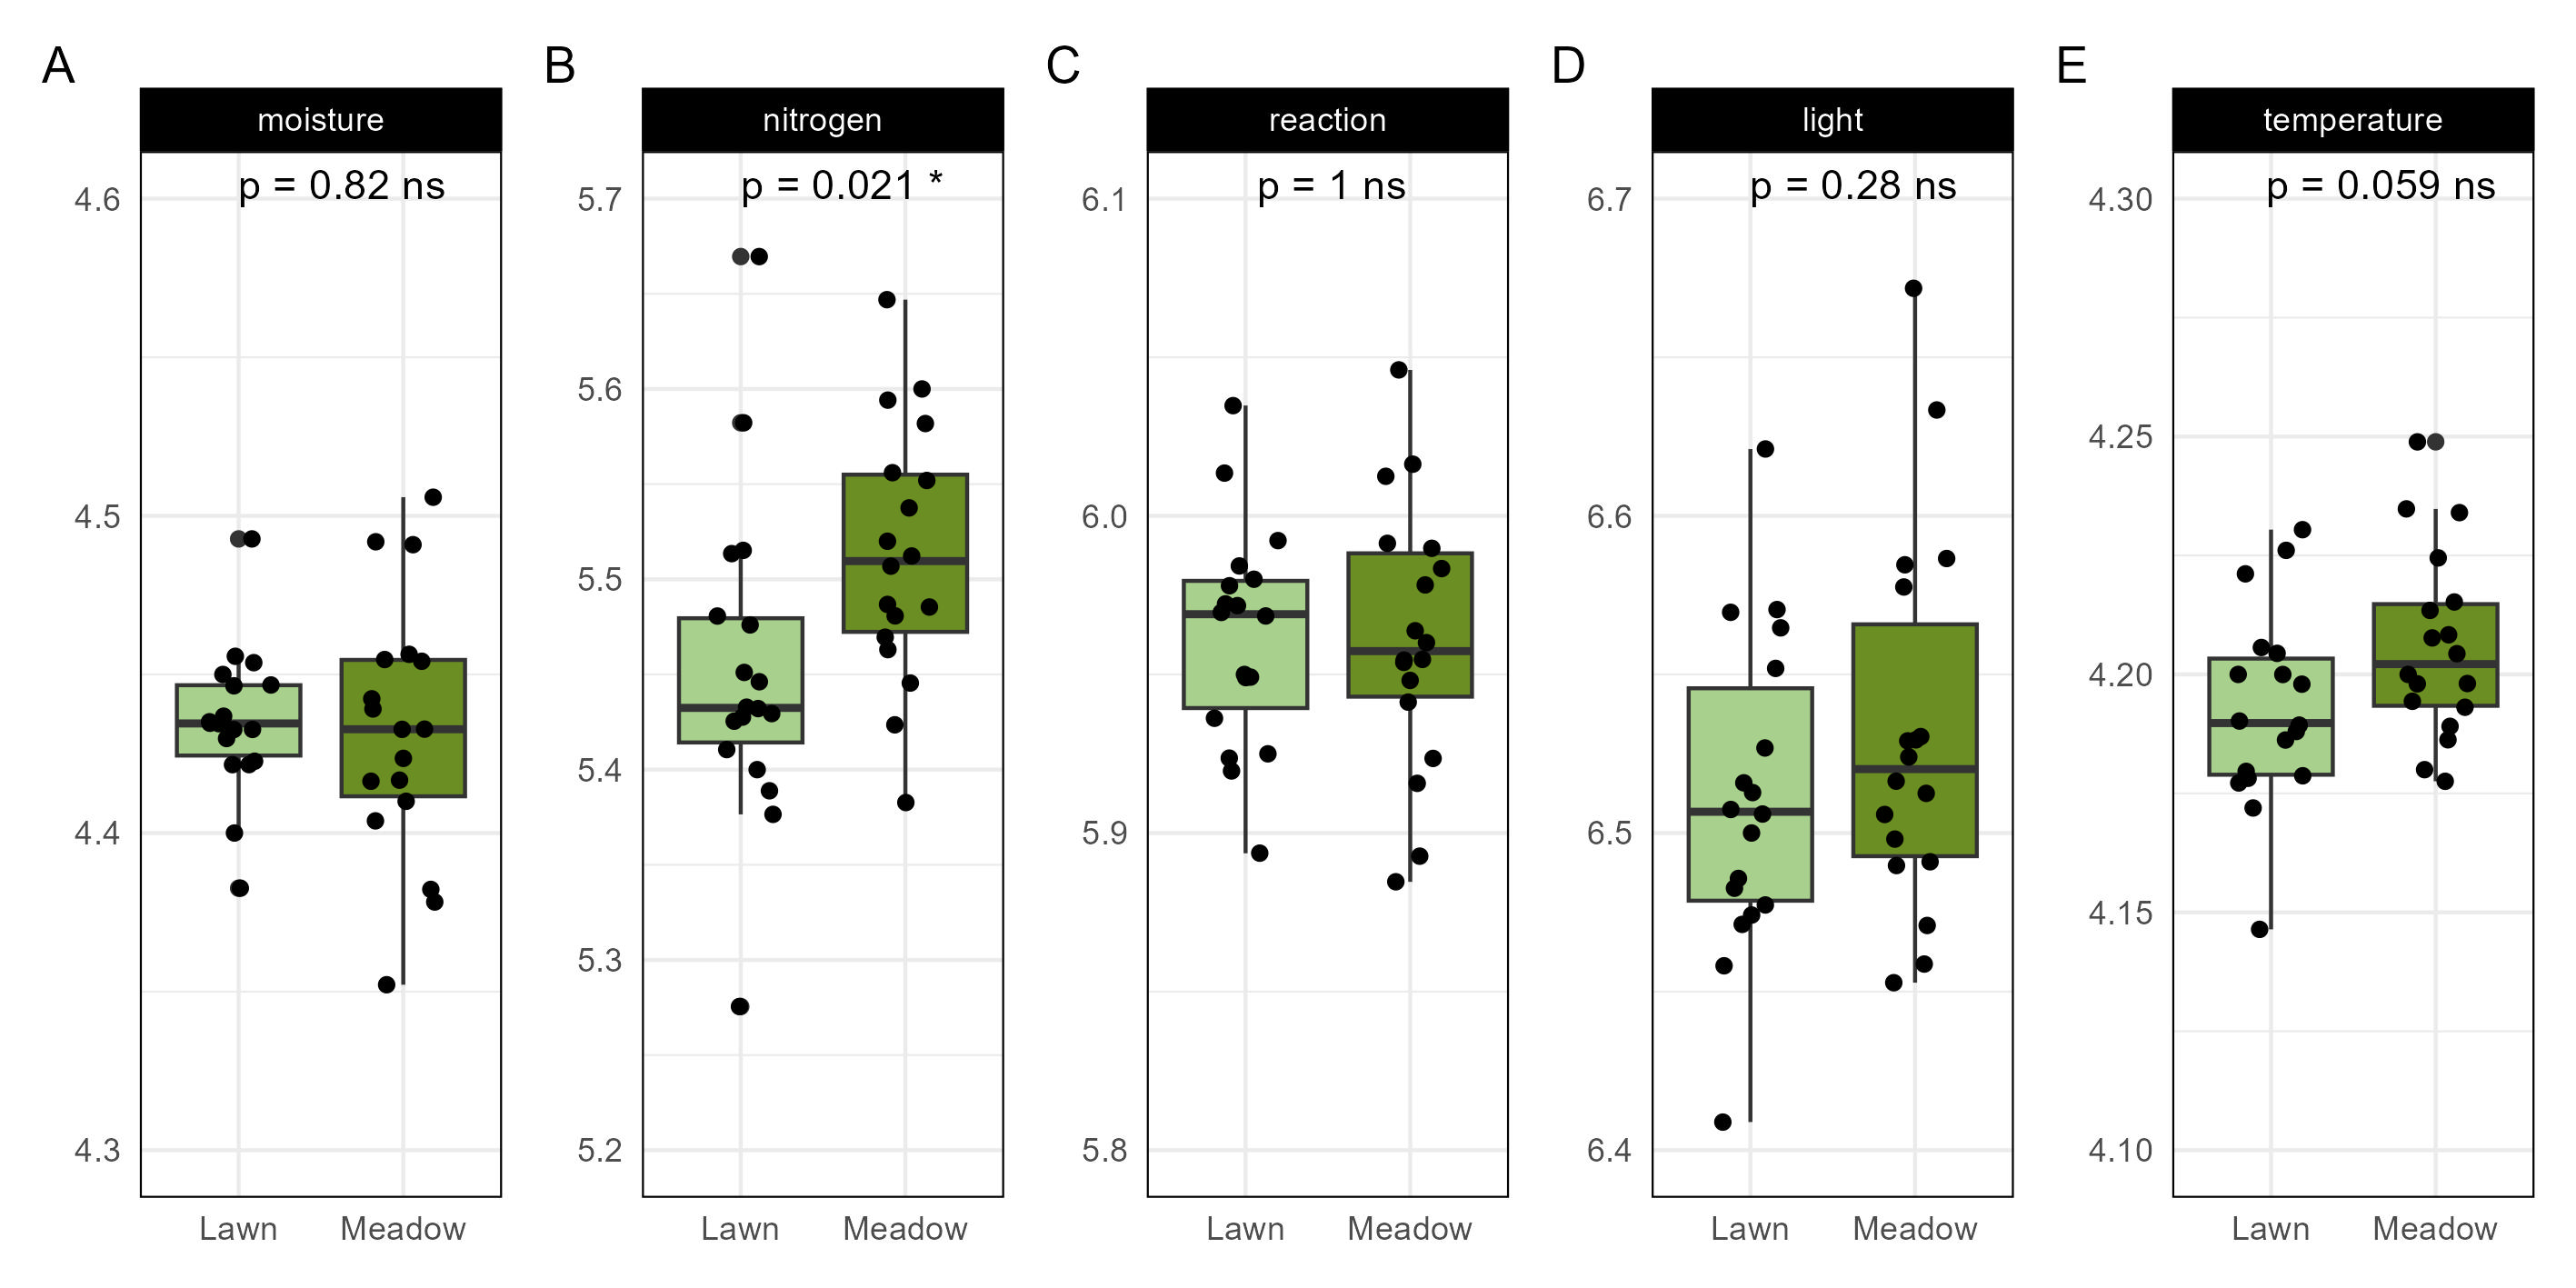
\includegraphics{plot_eiv_unweighted.jpg}

}

\caption{\label{fig-eiv_unweighted}Boxplots showing differences in
unweighted community means of ecological indicator values (EIVs) between
meadows and lawns. A significant difference was observed for nitrogen
values (B), with higher values in meadows. Temperature values tended to
be higher in meadows but were not significantly different.}

\end{figure}%

Regarding community-weighted means (CWMs) of functional traits, specific
leaf area (SLA) was significantly higher in meadows compared to lawns
(Figure~\ref{fig-traits_cwm}). No significant differences were found for
seed mass and canopy height between the two landuse types.

\begin{figure}[H]

\centering{

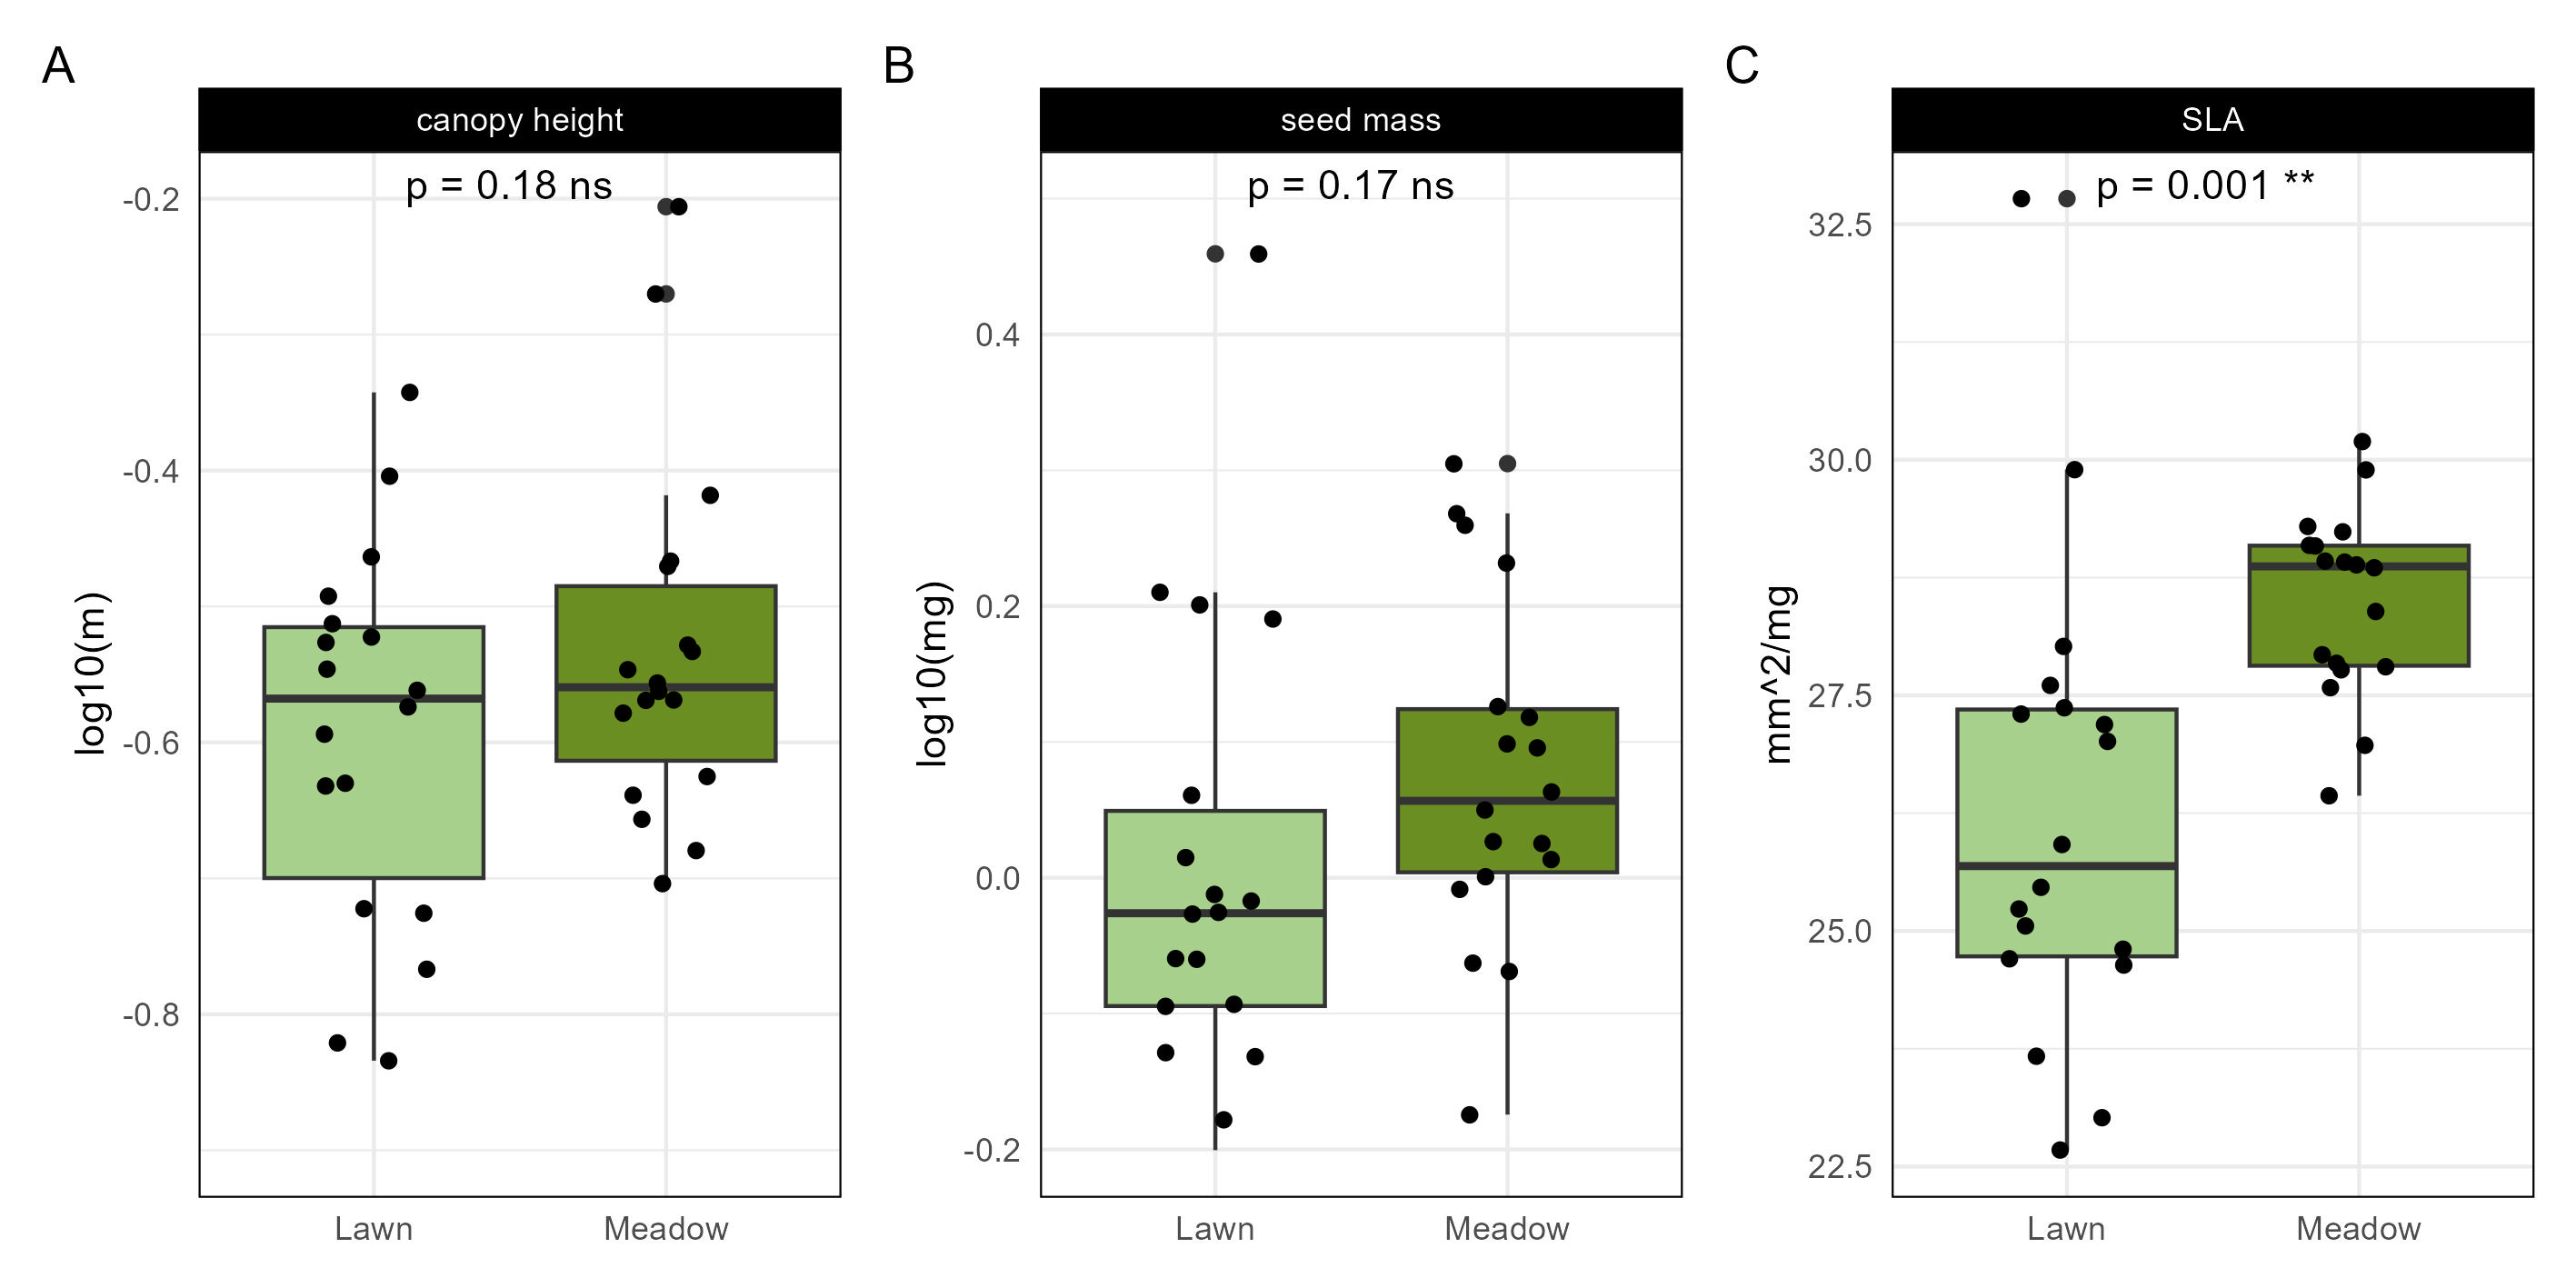
\includegraphics{plot_traits_cwm.jpg}

}

\caption{\label{fig-traits_cwm}Boxplots illustrating differences in
community-weighted means of functional traits ((A) canopy height, (B)
seed mass, and (C) specific leaf area) between meadows and lawns. A
significant difference was observed for SLA, with higher values in
meadows. No significant differences were found for canopy height and
seed mass.}

\end{figure}%

\subsection{References}\label{references}

\phantomsection\label{refs}
\begin{CSLReferences}{1}{0}
\bibitem[\citeproctext]{ref-dengler2023}
Dengler, Jürgen, Florian Jansen, Olha Chusova, Elisabeth Hüllbusch,
Michael P. Nobis, Koenraad Van Meerbeek, Irena Axmanová, et al. 2023.
{``Ecological Indicator Values for Europe (EIVE) 1.0.''}
\emph{Vegetation Classification and Survey} 4: 7--29.
\url{https://doi.org/10.3897/VCS.98324}.

\bibitem[\citeproctext]{ref-KleyerEtAl2008}
Kleyer, M., R. M. Bekker, I. C. Knevel, J. P. Bakker, K. Thompson, M.
Sonnenschein, P. Poschlod, et al. 2008. {``The LEDA Traitbase: A
Database of Life-History Traits of the Northwest European Flora.''}
\emph{Journal of Ecology} 96: 1266--74.
\url{https://doi.org/10.1111/j.1365-2745.2008.01430.x}.

\bibitem[\citeproctext]{ref-Laliberte2010}
Laliberté, Etienne, and Pierre Legendre. 2010. {``A Distance-Based
Framework for Measuring Functional Diversity from Multiple Traits.''}
\emph{Ecology} 91: 299--305.

\bibitem[\citeproctext]{ref-Laliberte2014}
Laliberté, Etienne, Pierre Legendre, and Bill Shipley. 2014. \emph{FD:
Measuring Functional Diversity from Multiple Traits, and Other Tools for
Functional Ecology}.

\bibitem[\citeproctext]{ref-RCoreTeam2025}
R Core Team. 2025. \emph{R: A Language and Environment for Statistical
Computing}. Vienna, Austria: R Foundation for Statistical Computing.
\url{https://www.R-project.org/}.

\end{CSLReferences}




\end{document}
